\documentclass[12pt]{article}

\usepackage{hyperref} % гиперссылки

\usepackage{tikz} % картинки в tikz
\usepackage{microtype} % свешивание пунктуации

\usepackage{array} % для столбцов фиксированной ширины

\usepackage{indentfirst} % отступ в первом параграфе

\usepackage{sectsty} % для центрирования названий частей
\allsectionsfont{\centering}

\usepackage{amsmath} % куча стандартных математических плюшек

\usepackage{comment} % добавление длинных комментариев

\usepackage[top=2cm, left=1.2cm, right=1.2cm, bottom=2cm]{geometry} % размер текста на странице

\usepackage{lastpage} % чтобы узнать номер последней страницы

\usepackage{enumitem} % дополнительные плюшки для списков
%  например \begin{enumerate}[resume] позволяет продолжить нумерацию в новом списке

\usepackage{caption} % что-то делает с подписями рисунков :)

\usepackage{qcircuit} % для рисовки квантовых диаграмм
\usepackage{physics} % бракеты

\usepackage{answers} % разделение условий и ответов в упражнениях

\usepackage{chessboard} % рисование шахматной доски


\usepackage{fancyhdr} % весёлые колонтитулы
\pagestyle{fancy}
\lhead{Демоническая оптимизация}
\chead{}
\rhead{КЛШ-2018}
\lfoot{}
\cfoot{}
\rfoot{\thepage/\pageref{LastPage}}
\renewcommand{\headrulewidth}{0.4pt}
\renewcommand{\footrulewidth}{0.4pt}



\usepackage{todonotes} % для вставки в документ заметок о том, что осталось сделать
% \todo{Здесь надо коэффициенты исправить}
% \missingfigure{Здесь будет Последний день Помпеи}
% \listoftodos — печатает все поставленные \todo'шки



\usepackage{booktabs} % красивые таблицы
% заповеди из докупентации:
% 1. Не используйте вертикальные линни
% 2. Не используйте двойные линии
% 3. Единицы измерения - в шапку таблицы
% 4. Не сокращайте .1 вместо 0.1
% 5. Повторяющееся значение повторяйте, а не говорите "то же"



\usepackage{fontspec} % что-то про шрифты?
\usepackage{polyglossia} % русификация xelatex

\setmainlanguage{russian}
\setotherlanguages{english}

% download "Linux Libertine" fonts:
% http://www.linuxlibertine.org/index.php?id=91&L=1
\setmainfont{Linux Libertine O} % or Helvetica, Arial, Cambria
% why do we need \newfontfamily:
% http://tex.stackexchange.com/questions/91507/
\newfontfamily{\cyrillicfonttt}{Linux Libertine O}

\AddEnumerateCounter{\asbuk}{\russian@alph}{щ} % для списков с русскими буквами
\setlist[enumerate, 2]{label=\asbuk*),ref=\asbuk*}

%% эконометрические сокращения
\DeclareMathOperator{\Cov}{Cov}
\DeclareMathOperator{\Corr}{Corr}
\DeclareMathOperator{\Var}{Var}
\DeclareMathOperator{\E}{E}
\def \hb{\hat{\beta}}
\def \hs{\hat{\sigma}}
\def \htheta{\hat{\theta}}
\def \s{\sigma}
\def \hy{\hat{y}}
\def \hY{\hat{Y}}
\def \v1{\vec{1}}
\def \e{\varepsilon}
\def \he{\hat{\e}}
\def \z{z}
\def \hVar{\widehat{\Var}}
\def \hCorr{\widehat{\Corr}}
\def \hCov{\widehat{\Cov}}
\def \cN{\mathcal{N}}



\usepackage[bibencoding = auto,
backend = biber,
sorting = none,
style=alphabetic]{biblatex}

\addbibresource{em1_pset_v2.bib}



% делаем короче интервал в списках
\setlength{\itemsep}{0pt}
\setlength{\parskip}{0pt}
\setlength{\parsep}{0pt}




\Newassociation{sol}{solution}{solution_file}
% sol --- имя окружения внутри задач
% solution --- имя окружения внутри solution_file
% solution_file --- имя файла в который будет идти запись решений
% можно изменить далее по ходу
\Opensolutionfile{solution_file}[all_solutions]
% в квадратных скобках фактическое имя файла

% магия для автоматических гиперссылок задача-решение
\newlist{myenum}{enumerate}{3}
% \newcounter{problem}[chapter] % нумерация задач внутри глав
\newcounter{problem}[section]

\newenvironment{problem}%
{%
\refstepcounter{problem}%
%  hyperlink to solution
     \hypertarget{problem:{\thesection.\theproblem}}{} % нумерация внутри глав
     % \hypertarget{problem:{\theproblem}}{}
     \Writetofile{solution_file}{\protect\hypertarget{soln:\thesection.\theproblem}{}}
     %\Writetofile{solution_file}{\protect\hypertarget{soln:\theproblem}{}}
     \begin{myenum}[label=\bfseries\protect\hyperlink{soln:\thesection.\theproblem}{\thesection.\theproblem},ref=\thesection.\theproblem]
     % \begin{myenum}[label=\bfseries\protect\hyperlink{soln:\theproblem}{\theproblem},ref=\theproblem]
     \item%
    }%
    {%
    \end{myenum}}
% для гиперссылок обратно надо переопределять окружение
% это происходит непосредственно перед подключением файла с решениями





\begin{document}

\tableofcontents{}

\section*{Цель}


\newpage
\section{Забери камень}


\begin{problem}

Четыреста лет назад, в 1612 г. в Лионе появилась книга поэта и математика Баше де Мезирьяка
(Claude Gaspar Bachet de M\'eziriac
\footnote{Баше де Мезирьяк перевел с греческого на латынь Арифметику Диофаната,
на полях которой Ферма сформулировал свою великую теорему})
«Занимательные и приятные числовые задачи» (Probl\`emes plaisants et d\'electables qui se font par les nombres).
В ней была предложена следующая игра. Двое по очереди называют числа от 1 до 10, выигрывает тот,
кто первым доведет сумму до 100. В чью пользу эта игра?

Ссылка на переиздание 1884 года \url{http://cnum.cnam.fr/DET/8PY45.html}, задача 22.

\begin{sol}

\end{sol}
\end{problem}



\begin{problem} Цзяньшинцзы «Выбирание камней»

Древний Китай. Две кучки камней. Два игрока ходят по очереди.
За один ход можно забрать либо произвольное число камней из одной кучки,
либо одинаковое число камней из обеих. В одной кучке 5, а в другой — 8 камней.

Кто выигрывает при правильной игре?

\begin{sol}

\end{sol}
\end{problem}


\begin{problem} «Одинокий ферзь»

Шахматная доска, одинокий раненый ферзь стоит на h6.
Раненый ферзь как и ферзь может двигаться на любое число клеток,
но только влево или вниз, или влево-вниз. Двое игроков ходят по очереди,
тот кто переставит ферзя на а1 выиграл.
\begin{enumerate}
\item В чью пользу эта игра? Если в пользу первого, то с какого хода следует начать игру?
\item Какие позиции на доске являются проигрышными и проигрышными, если ферзь очень
сильно ранен и больше чем на два шага пойти не может?
\item Найди 10 отличий игры «Одинокий ферзь» от игры «Цзяньшинцзы».
\end{enumerate}

\def\mylist{Qh6}
\setchessboard{setpieces=\mylist,showmover=false}
\chessboard

\begin{sol}

\end{sol}
\end{problem}

\begin{problem} «Набери чет»

В кучке 135 камней, двое по очереди забирают себе от 1 до 4 камней.
Выигрывает тот, кто к концу игры наберет четное число камней.

Кто выигрывает при правильной игре?

\begin{sol}

\end{sol}
\end{problem}


\begin{problem}

В кучке 147 камней, Полина и Василий по очереди берут камни.
Полина начинает первой. Выигрывает тот, кто возьмёт последний камень.
Полина может взять 1, 4 или 5 камней, а Василий — 1, 3 или 4 камня.

\begin{enumerate}
  \item Кто выигрывает при правильной игре?
  \item Как изменится результат, если Василий может брать 1, 3, 4 или 20 камней?
  \item Как изменится результат, если Василий может брать 1, 3, 4 или 6 камней?
\end{enumerate}

\begin{sol}

\end{sol}
\end{problem}



\begin{problem} Опустошай и разделяй!

Есть две коробочки. В каждой из них лежит некоторое количество камешков.
Игроки ходят по очереди.
За один ход игрок выбрасывает содержимое одной из коробочек,
и затем делит содержимое другой между двумя коробочками.
Как минимум один камешек должен оставаться в каждой коробочке.
Проигрывает тот, кто не может сделать ход по правилам.

Найди все выигрышные позиции.
\begin{sol}

\end{sol}
\end{problem}


\begin{problem} Опустошай и разделяй без равенства!

Есть две коробочки. В каждой из них лежит некоторое количество камешков.
Игроки ходят по очереди.
За один ход игрок выбрасывает содержимое одной из коробочек,
и затем делит содержимое другой между двумя коробочками.
\textbf{Поровну делить нельзя!}
Как минимум один камешек должен оставаться в каждой коробочке.
Проигрывает тот, кто не может сделать ход по правилам.

Каковы есть оптимальные ходы в позиции $7$ и $9$ камешков?
\begin{sol}

\end{sol}
\end{problem}


\newpage
\section{Дерево игры}

\begin{problem} Кортес

Кортес с бандой головорезов высадился на берегу.
Кортес выбирает, нападать ли на деревушку или нет.

Местная деревушка может либо сразу перейти в подчинение Кортеса, либо принять бой.
Если деревушка примет бой, то выбор появится у Кортеса: либо драться до победного конца,
либо после первых потерь бежать на кораблях обратно.

Ценность деревушки для Кортеса — одна единица, ценность собственных головорезов — 2 единицы.
Если Кортес будет драться до конца, то деревушка будет взята,
но большинство головорезов погибнет в бою. Для жителей деревушки — главное остаться в живых,
сохранить при этом независимость, конечно, желательно.

\begin{enumerate}
  \item Нарисуй дерево игры и найди обратно-индукционный исход.
  \item Нарисуй дерево игры и найди обратно-индукционный исход в случае, если Кортес сжёг корабли.
\end{enumerate}

\begin{sol}

\end{sol}
\end{problem}

\begin{problem} Рулетки

Есть три рулетки: на первой равновероятно выпадают числа 2, 4 и 9; на второй — 1, 6 и 8;
на третьей — 3, 5 и 7. Сначала первый игрок выбирает рулетку себе,
затем второй игрок выбирает рулетку себе из двух оставшихся.
После этого рулетки, выбранные игроками, запускаются, и случай определяет победителя.
Победителем считается тот, чья рулетка покажет большее число.

Победитель получает от проигравшего 100 рублей.

В чью пользу эта игра?

\begin{sol}
Вероятность выигрыша для второго игрока — $5/9$.
\end{sol}
\end{problem}


\section{Определение высоты здания}

\section{Подбрасывание кубики}

\section{ООР и РОО}

\section{ООР и РОО с правом выбора}

\section{Ним-стоимость}

\section{Ним-подобные игры}

\section{Задача о разборчивой невесте}

\begin{problem}
Задача о Разборчивой Невесте, Secretary problem

К Разборчивой невесте выстроилась длинная-длинная вереница из потенциальных женихов.
\footnote{Докторская диссертация член-корреспондента РАН Бориса Березовского
«Разработка теоретических основ алгоритмизации принятия предпроектных решений и их применения»
является обобщением задачи о разборчивой невесте, \url{http://en.wikipedia.org/wiki/Secretary_problem}}
Разборчивая невеста хочет выбрать самого богатого из них и только его!
Потенциальные женихи заходят к Разборчивой невесте по одному в случайном порядке.
Невеста неплохо разбирается в богатстве и всегда может ранжировать всех, с кем она общалась,
по величине богатства. Когда к Разборчивой невесте приходит очередной претендент,
она должна сразу принять решение: выбрать данного кандидата или перейти к следующему.
Вернуться к предыдущим кандидатам невозможно — они обижаются и уезжают.

\begin{enumerate}
\item Как выглядит оптимальная стратегия Разборчивой невесты? Чему равна вероятность выбора самого богатого жениха Разборчивой невестой?
\item Подруга-дурнушка Разборчивой невесты хочет выбрать второго по богатству жениха и только его!
Как выглядит её оптимальная стратегия?
Чему равна вероятность выбора второго по богатству жениха Подругой-дурнушкой?
\end{enumerate}

\begin{sol}
Пусть:

$n$ - количество потенциальных женихов,

$t$ - номер шага, на котором находится невеста,

$G_t$ - вероятность того, что $t$-ый жених лучше всех предыдущих,

$F_t$ - вероятность того, что пропустив $t$ женихов и дальше пользуюясь оптимальной
стратегией (предполагается, что невеста будет пользоваться предложенной стратегией с $t+1$
шага), невеста выберет в мужья самого богатого.

Определим вероятность $G_t$. Очевидно, что $G_n = 1$. Тогда вероятность того, что $n$-ый жених будет лучше всех предыдущих, равна  $\frac{1}{n}$ $\Rightarrow$ $G_{n-1}=1-\frac{1}{n}=\frac{n-1}{n}$ – вероятность "победы" на $n-1$ шаге. Пользуемся дальше подобной логикой. $\frac{1}{n-1}$ – вероятность того, что $n-1$ жених лучше $n-2\Rightarrow$ вероятноть того, что $n-1$ будет не лучше $n-2$ равна $1-\frac{1}{n-1}=\frac{n-2}{n-1}\Rightarrow G_{n-2}= \frac{1}{n-1}\cdot 0+\frac{n-2}{n-1}\cdot G_{n-1}=\frac{n-2}{n}$. Используя метод математической индукции получаем, что $G_t=\frac{t}{n}$.

Теперь найдём $F_t$. Для этого стоит уточнить, что Разборчивая невеста будет пользоваться оптимальной стратегией с $t+1$ шага, то есть всех предыдущих женихов она сразу отвергает. И ещё очень важно заметить, что вероятность успеха невесты в её нелёгком деле не превышает величины $F_t \Rightarrow F_{t+1} \le F_t \Rightarrow F_t$ – убывающая последовательность. Из всего вышесказанного делаем вывод, что $F_n = 0$, так как отвергнув последнего жениха, невеста останется одна $\Rightarrow F_{n-1}=\frac{1}{n}$ - вероятность, что $n$-ый жених лучше всех. Тогда $F_{n-2}=\frac{1}{n-1}\cdot\frac{n-1}{n}+\frac{n-2}{n-1}\cdot\frac{1}{n}=\frac{(n-2)+(n-1)}{n(n-1)}$. В данном случае сразу найти итоговый $F_t$ затрруднительно, поэтому рассмотрим величину $\frac{F_t}{G_t}$, тем более нам всё равно придётся сравнивать дальше эти величины. Получается, что $\frac{F_{n-2}}{G_{n-2}}=\frac{1}{n-1}+\frac{1}{n-2}$ $\Rightarrow$ по методу математической индукции $F_t = \frac{t}{n} \cdot (\frac{1}{t}+\frac{1}{t+1}+\ldots +\frac{1}{n-1})$.

Перейдём к самой стратегии. Представим, что $F_t$ и $G_t$ непрервыные функции(хотя это не так, потому что они зависят от целых чисел). Тогда $F_t$ - монотонно убывающая функция, а $G_t$ монотонно возрастающая и изобразить их в осях $t, P$, где $P$ - вероятность и $E(G_t)=E(F_t)=[0;1]$ ($E$ - область значения), то найдётся такая точка $T$, в которой эти графики пересекутся $\Rightarrow$ надо найти ближайшее целое $t_1$, до которого невеста пропустит всех женихов, а дальше остановится на первом же, который луше всех предыдущих.

Для того, чтобы найти это оптимальное $t_1$, необходимо рассмотреть соотношение $\frac{F_t}{G_t}$ и сравнить его с $1$. Получается, что $\frac{F_t}{G_t}= \frac{1}{t}+\frac{1}{t+1}+\ldots +\frac{1}{n-1}$, для $t \ge t_1$.

Предположим, что $n, t$ - достаточно большие числа, которые позволят нам перейти к рассматриванию функций. Заметим, что если нарисовать график $y=\frac{1}{x}$, отметить точки $t, t+1,\ldots , n$ и нарисовать прямоугольники с длиной соответствующей  $\frac{1}{t}, \frac{1}{t+1},\ldots ,\frac{1}{n}$ и шириной $1$, то сумма площадей этих прямогольников будет соответствовать $S = \frac{1}{t}+\frac{1}{t+1}+\ldots +\frac{1}{n-1}$.

Если произвети сжатие и растяжение функции $y=\frac{1}{x}$ в t раз, величина $\frac{1}{t}$ станет очень маленькой $\Rightarrow$ сумма площадей прямоугольников практически в точности будет соответствовать площади под графиком на отрезке $[t, n]$. Заметим, что равенство $S(xy)=S(x)+S(y)$ выполняется для всех $x, y>1$, что соответсвует одмому из свойств логарифмов $\Rightarrow S(x)=log_a(x)\Rightarrow$ для обратой функциии будет выполняться $H(x+y)=H(x)*H(y)\Rightarrow$ это показательная функция $H(x)= a^x$. В итоге получаем, что $a$ – это то самое число, которое нам надо узнать для того, чтобы найти $S(x)$. Так как $H(1)=a \Rightarrow F(a)=1 \Rightarrow$ рассмотрим различные значение пложади под $y=\frac{1}{x}$. $S(2)<1\Rightarrow a>2, S(2,5)<1 \Rightarrow a>2,5 , S(3)>1 \Rightarrow a<3 \Rightarrow$ интуитивно понятно, что $a = e$.
В итоге имеем, что $\frac{F_t}{G_t}=1 \Leftrightarrow \frac{n}{t}=e \Leftrightarrow \frac{t}{n}=\frac{1}{e}\Rightarrow F_t=G_t=\frac{t}{n}=\frac{1}{e}\Rightarrow$ вероятность «успеха» невесты найти самого богатого $\frac{1}{e}\approx 0,368$.

А оптимальная стратегия такова: пропустить $\approx 36,8\%$ женихов и выбрать первого же, который будет лучше всех своих предшественников.
\end{sol}

\end{problem}

\section{Труэль}


\begin{problem}
Труэль

Три игрока решили стреляться ради самой красивой девушки и организуют труэль (дуэль для трёх игроков).  Игроки стреляют по очереди, $A$-$B$-$C$-$A$-\ldots. Каждый из игроков может либо целиться в одного из противников, либо стрелять в воздух. Вероятности попадания равны $p_a=0.6$, $p_b=0.5$ и $p_c=0.4$, соответственно. Игра продолжается до определения единственного победителя, он и получает девушку в жёны.

\begin{enumerate}
\item Как выглядит оптимальная стратегия каждого игрока?
\item Чему равные вероятности выиграть для каждого игрока?
\end{enumerate}

\begin{sol}
\textbf{Оптимальные стратегии}

Оптимальная стратегия игрока А (вероятность попадания 0.6) - в любом случае будет стрелять в противника, так как его вероятность попасть больше, чем у остальных, а вероятность, что попадут в него, меньше.

Оптимальная стратегия игрока С (вероятность попадания 0.4) - стрелять в воздух до того момента, как в игре останутся два игрока (С + А/В). Так он дает сильным игрокам возможность "разобраться" друг с другом, и если один убивает другого, то следующим ходом он первым имеет возможность уничтожить оставшегося ( пусть и с небольшой вероятностью). В противном случае, если он убивает А, то следующим ходом с большой вероятность В убьет его самого.

Оптимальная стратегия игрока В (вероятность попадания 0.5) совпадает со стратегией игрока А (может быть, В и выгодно бы было отклонятся, но он понимает стратегию С и в таком случае не будет стрелять в воздух).

\textbf{Решение по дереву вероятностей}

\begin{figure*}
    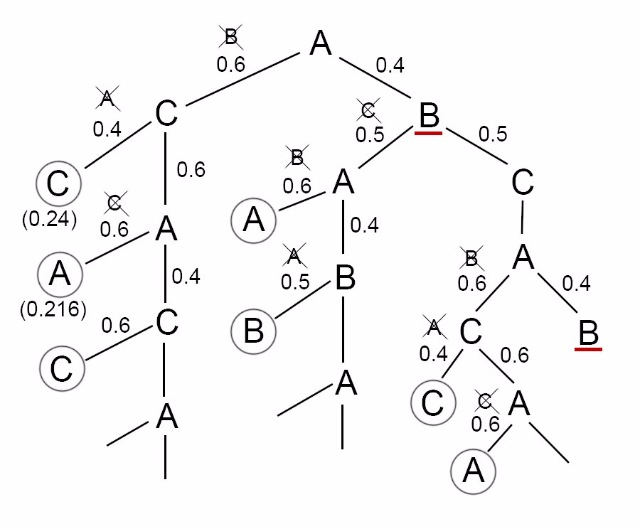
\includegraphics[width=10cm]{images/truel_task37.jpg}
\end{figure*}
\begin{enumerate}
\item Если первым выстрелом А убил В (с вероятностью 0.6), то шанс победить остается у А и у С. Вероятность, что дальше С попадет в цель своим первым выстрелом и победит = 0.24. Если же С промахивается, а следующим ходом А его убивает, то А побеждает с вероятностью 0.216. Если А промахивается, то исход дуэли решает С и цикл повторяется. Можно заметить, что вероятность победы любого из них - сумма бесконечно убывающей геометрической прогресии.

$\P(\text{победа C})= \frac{0.24}{1-0.24} = 0.32$

$\P(\text{победа A}) = \frac{0.216}{1-0.24} = 0.28$
\item Если первым выстрелом А не убивает В, то

а) следующим ходом В убивает С и победа разыгрывается между А и В;

б) В не убивает С, тогда (С стреляет в воздух) либо А убивает В, либо промахивается, и ход опять падает на В (при этом все живы) - цикл повторяется.

а) $\P(\text{победа A}) = \frac{0.12}{1-0.2} = 0.15$

$\P(\text{победа B}) = \frac{0.04}{1-0.2} = 0.05$

б) Теперь можно учесть повтор цикла для вероятности А и В (случай, когда А промахнулся и ход опять перешел В)

$\P(\text{победа A}) = \frac{0.15}{1-0.2} = 0.19$

$\P(\text{победа B}) = \frac{0.05}{1-0.2} = 0.06$

Если же А сразу убивает В, то (учитывая все циклы)

$\P(\text{победа A}) = \frac{\frac{0.0432}{1-0.24}}{1-0.2} = 0.07$

$\P(\text{победа C}) = \frac{\frac{0.048}{1-0.24}}{1-0.2} = 0.08$

\textbf{Проверим сумму вероятностей}: $0.32 + 0.28 + 0.19 + 0.06 + 0.07 + 0.08 = 1 $

\textbf{Результат}:

$\P(\text{победит A}) = 0.28 + 0.19 +0.07 = 0.54$

$\P(\text{победит B}) = 0.06$

$\P(\text{победит С}) = 0.32 + 0.08 = 0.4$
\end{enumerate}
\end{sol}

\end{problem}


\section{Задача о делении ставки}

\begin{problem}
У домашнего учителя Алексея Ивановича один фридрихсдор.
Перед ним обычная колода в 52 карты.
Перед открытием каждой карты Алексей Иванович выбирает,
какую долю своего богатства, от нуля до единицы, поставить на цвет следующей карты.
Карты бывают двух цветов: чёрные и красные. Например, у Алексея Ивановича есть такая стратегия:
не ставить ничего вплоть до последней карты и затем поставить весь рубль на нужный цвет.
Такая стратегия гарантированно удвоит его богатство.

Найдите стратегию, которая максимизирует гарантированный выигрыш Алексея Ивановича.
Чему равен этот максимальный гарантированный выигрыш?
\begin{sol}

\end{sol}

\end{problem}



\section{Сходитесь!}

\begin{problem}
Примирение невозможно, и потому Андрей и Борис решаются на дуэль.

\begin{sol}

\end{sol}

\end{problem}



\begin{problem}
Истеричная певица

Начинающая певица дает концерты каждый день. Каждый ее концерт приносит продюсеру 0.75 тысяч евро. После каждого концерта певица может впасть в депрессию с вероятностью 0.5. Самостоятельно выйти из депрессии певица не может. В депрессии она не в состоянии проводить концерты. Помочь ей могут только цветы от продюсера. Если подарить цветы на сумму $0\le x\le 1$ тысяч евро, то она выйдет из депрессии с вероятностью $\sqrt{x}$.

Какова оптимальная стратегия продюсера? Продюсер максимизирует текущую ожидаемую ценность певицы.

\begin{sol}
  Рассмотрим совершенно конкурентный невольничий рынок начинающих певиц. Певицы в хорошем настроении продаются по $V_1$, в депрессии — по $V_2$. Получаем систему уравнений:
\[
\begin{cases}
  V_1 = 0.75 + (0.5 V_1 + 0.5 V_2) \\
  V_2 = \max_x \sqrt{x}V_1 + (1 - \sqrt{x})V_2 - x
\end{cases}
\]
Оптимизируем и получаем, $x^* = (V_1 - V_2)^2/4$. Из первого уравнения находим $(V_1 - V_2)/2=0.75$.
\end{sol}

\end{problem}


задача о змее горыныче?




\section{Биномиальная модель цены акции}

\section{Опционы американского типа}


\section{Идеи}

\begin{enumerate}
  \item Начинай с хвоста
  \item Сделай первый шаг
  \item Цена позиции
  \item MR=MC, сформулировать словами (!)
\end{enumerate}


\section{Лог}

\begin{enumerate}
  \item Было 8 школьников, 9-10 класс. Решили 1.1. Сформулировали принципы.
  За $+$ обязательно найдётся $-$, за $-$ идут только плюсы.
  Рассчитываем на 1 шаг вперёд, и далее пользуемся уже рассчитанным.
  Игроки рациональны. Начинай с хвоста. Затем 1.3, 1.4. и 1.5.
\end{enumerate}



\Closesolutionfile{solution_file}

% для гиперссылок на условия
% http://tex.stackexchange.com/questions/45415
\renewenvironment{solution}[1]{%
         % add some glue
         \vskip .5cm plus 2cm minus 0.1cm%
         {\bfseries \hyperlink{problem:#1}{#1.}}%
}%
{%
}%

\section{Решения}
\protect \hypertarget {soln:1.1}{}
\begin{solution}{{1.1}}
  $\P(X=1)=3/5$, $\P(X=2)=3/10$, $\P(X=3)=1/10$, $\E(X)=1.5$
\end{solution}
\protect \hypertarget {soln:1.2}{}
\begin{solution}{{1.2}}
\end{solution}
\protect \hypertarget {soln:1.3}{}
\begin{solution}{{1.3}}
\end{solution}
\protect \hypertarget {soln:1.4}{}
\begin{solution}{{1.4}}
   N 3 4 5

  2/8 3/8 3/8
\end{solution}
\protect \hypertarget {soln:2.1}{}
\protect \hypertarget {soln:2.2}{}
\protect \hypertarget {soln:2.3}{}
\protect \hypertarget {soln:2.4}{}
\protect \hypertarget {soln:3.1}{}
\begin{solution}{{3.1}}
\end{solution}
\protect \hypertarget {soln:3.2}{}
\begin{solution}{{3.2}}
\end{solution}
\protect \hypertarget {soln:10.1}{}
\begin{solution}{{10.1}}
  
\end{solution}
\protect \hypertarget {soln:11.1}{}
\begin{solution}{{11.1}}
  
\end{solution}
\protect \hypertarget {soln:11.2}{}
\begin{solution}{{11.2}}
  Например, $CNOT = \ketbra{00}{00} + \ketbra{01}{01} + \ketbra{10}{11} + \ketbra{11}{10}$.
\end{solution}




\end{document}
